\section{Auswertung}
\label{sec:Auswertung}

\subsection{Spannungskurven bei unterschiedlichen Phasen.}
Es wird eine Signalspannung von 25,6 V mit einer Frequenz von 2 kHz angelegt. Als
Referenzsignal dient eine Spannung gleicher Frequenz mit einer Amplitude von
2,32 V.
Bei unterschiedlichen Phaseneinstellungen des Phase Shifters ergeben sich
die in Abbildung \ref{fig:logos} zu sehenden Spannungen am Detektor.
Zu erkennen sind die erwarteten Halbwellen (negative bzw. positive Halbwellen sind umgeklappt),
die anschließend bei der zeitlichen Mittelung im Tiefpass einen nicht verschwindenden
Spannungsanteil liefern sollten.
Bei Variation der Phase verschieben sich die Kurven jeweils,
bis sie bei einer Phasendifferenz von 180° umklappen. Im Bereich von 0°-180° erhält
man also nur negative Halbwellen und im Bereich von 180°-360° nur positive.
In Abbildung \ref{fig:logosv} ist ein identisches Verhalten zu beobachten.
Jedoch ist auch zusätzlich das Rauschen anhand des unstetigen Verlaufs der Kurven zu
erkennen.
\begin{figure}
  \centering
  \begin{subfigure}{0.48\textwidth}
    \centering
    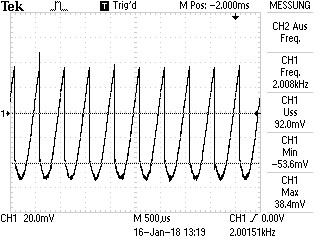
\includegraphics[height=4cm]{phase0.jpg}
    \caption{Phase 0.}
    \label{fig:phase0}
  \end{subfigure}
  \begin{subfigure}{0.48\textwidth}
    \centering
    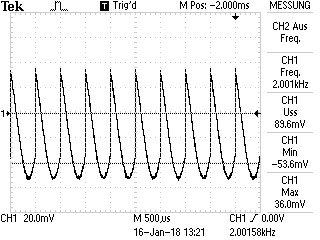
\includegraphics[height=4cm]{phase90.jpg}
    \caption{Phase 90.}
    \label{fig:phase90}
  \end{subfigure}
  \begin{subfigure}{0.48\textwidth}
    \centering
    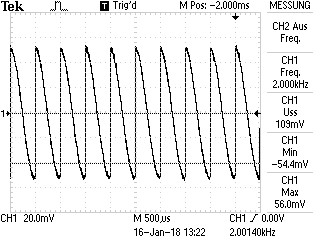
\includegraphics[height=4cm]{phase135.jpg}
    \caption{Phase 135.}
    \label{fig:phase135}
  \end{subfigure}
  \begin{subfigure}{0.48\textwidth}
    \centering
    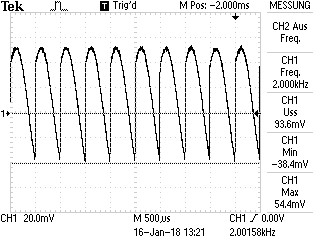
\includegraphics[height=4cm]{phase180.jpg}
    \caption{Phase 180.}
    \label{fig:phase180}
  \end{subfigure}
  \begin{subfigure}{0.48\textwidth}
    \centering
    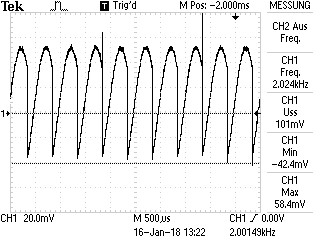
\includegraphics[height=4cm]{phase270.jpg}
    \caption{Phase 270.}
    \label{fig:phase270}
  \end{subfigure}
  \caption{Spannung am Detektor bei unterschiedlichen Phaseneinstellungen.}
  \label{fig:logos}
\end{figure}

\begin{figure}
  \centering
  \begin{subfigure}{0.48\textwidth}
    \centering
    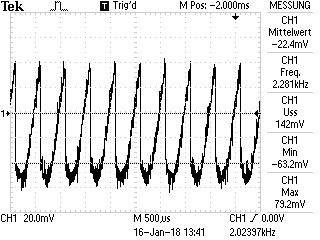
\includegraphics[height=4cm]{phase0v.jpg}
    \caption{Phase 0.}
    \label{fig:phase0v}
  \end{subfigure}
  \begin{subfigure}{0.48\textwidth}
    \centering
    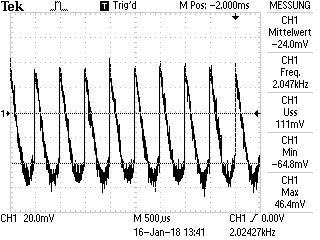
\includegraphics[height=4cm]{phase90v.jpg}
    \caption{Phase 90.}
    \label{fig:phase90v}
  \end{subfigure}
  \begin{subfigure}{0.48\textwidth}
    \centering
    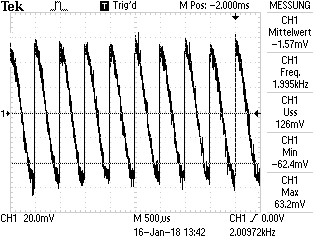
\includegraphics[height=4cm]{phase135v.jpg}
    \caption{Phase 135.}
    \label{fig:phase135v}
  \end{subfigure}
  \begin{subfigure}{0.48\textwidth}
    \centering
    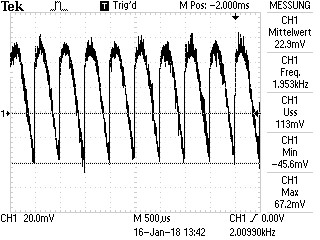
\includegraphics[height=4cm]{phase180v.jpg}
    \caption{Phase 180.}
    \label{fig:phase180v}
  \end{subfigure}
  \begin{subfigure}{0.48\textwidth}
    \centering
    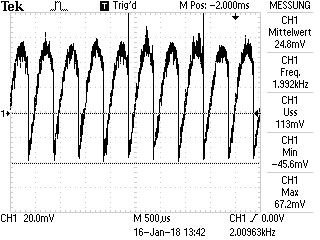
\includegraphics[height=4cm]{phase270v.jpg}
    \caption{Phase 270.}
    \label{fig:phase270v}
  \end{subfigure}
  \caption{Spannung am Detektor bei unterschiedlichen Phaseneinstellungen und Störsignal.}
  \label{fig:logosv}
\end{figure}

\FloatBarrier

\subsection{Messung von verrauschten Signalen in Abhängigkeit von der Phase}

Die gemessenen Spannungen mit und ohne Rauschen, in Abhängigkeit von der Phase $\phi$, werden in Tabelle 1 dargestellt.

\begin{table}[H]
  \centering
  \caption{Spannungen in Abhängigkeit von der Phase}
  \label{tab:Phase}
  \begin{tabular}{c c c}
    \toprule
    $\phi/$grad  &  $U_{out}/$mV &  $U_v/$mV \\
    \midrule
    0     &  -21,8   &  -22,0 \\
    30    &  -29,7   &  -30,0 \\
    60    &  -30,2   &  -30,5 \\
    90    &  -23,4   &  -23,4 \\
    120   &  -11,9   &  -11,4 \\
    150   &   11,4   &   12,2 \\
    180   &   23,3   &   23,5 \\
    210   &   31,1   &   31,7 \\
    240   &   31,4   &   32,1 \\
    270   &   24,8   &   25,0 \\
    300   &   13,1   &   12,9 \\
    \bottomrule
  \end{tabular}
\end{table}

Die Messwerte der nicht verrauschten Spannungen werden gegen die Phase aufgetragen. Eine Ausgleichsfunktion mit der Form
$A \cos{\phi + B} + C$ mit den Parametern $A, B ,C$ wird erstellt und ist in Abbildung \ref{fig:plot} zu sehen.

(Alle Plots werden mit Python erstellt und alle Fehler mit Python berechnet.)



\begin{figure}[H]
  \centering
  \includegraphics{plot.pdf}
  \caption{Nicht verrauschte Spannungen in Abhängigkeit von der Phase}
  \label{fig:plot}
\end{figure}

Die Parameter betragen:
\begin{align*}
  A &= \SI{-32.6(8)}{\milli\volt} \\
  B &= \SI{33.72(2)}{} \\
  C &= \SI{1.0(6)}{\milli\volt}
\end{align*}


Mit dem verrauschtem Signal wird analog vorgegangen. Die Messwerte und die Ausgleichsfunktion ist sind in Abbildung \ref{fig:plot2} dargestellt.

\begin{figure}[H]
  \centering
  \includegraphics{plot2.pdf}
  \caption{Nicht verrauschte Spannungen in Abhängigkeit von der Phase}
  \label{fig:plot2}
\end{figure}


Die Parameter der Funktion $D \cos{\phi + E} + F$ betragen:
\begin{align*}
  D &= \SI{-32.9(8)}{\milli\volt} \\
  E &= \SI{33.73(3)}{} \\
  F &= \SI{1.2(6)}{\milli\volt}
\end{align*}



\subsection{Messung eines verrauschten Lichtsignals}
Die gemessene Spannung $U$ der Photodiode, in Abhängigkeit von dem Abstand $r$, wird in Tabelle 2 dargestellt.

\begin{table}[H]
  \centering
  \caption{Spannungen in Abhängigkeit von dem Abstand}
  \label{tab:Phase}
  \begin{tabular}{c c}
    \toprule
    $r/$cm  &  $U/$mV \\
    \midrule
     2,5   &    336    \\
     3     &    320    \\
     4     &    280    \\
     5     &    232    \\
     6     &    178    \\
     7     &    118    \\
     8     &    52,8    \\
     9     &    40,0    \\
    10     &    30,4    \\
    15     &    18,8    \\
    20     &    12,2    \\
    25     &    8,8     \\
    30     &    6,4     \\
    40     &    4,6     \\
    50     &    2,8     \\
    60     &    2,6     \\
    70     &    2,5     \\
    \bottomrule
  \end{tabular}
\end{table}

Der Logarithmus der Spannung wird gegen den Logarithmus des Abstands aufgetragen. Eine Ausgleichsfunktion mit der Form $B \cdot x + C$ wird verwendet. Gemäß dem
Abstandsgesetz für Kugelwellen, ist eine Steigung $B = 2$ zu erwarten.

\begin{figure}[H]
  \centering
  \includegraphics{plot4.pdf}
  \caption{Spannungen in Abhängigkeit von dem Abstand}
  \label{fig:plot4}
\end{figure}

Der Parameter $B$ beträgt $B= -1,67 \pm 0.07$.
